\documentclass{article}
\usepackage[nonatbib]{nips} 
\usepackage{amsmath}
\usepackage{graphicx}
\usepackage{amssymb}
\usepackage{listings}
\graphicspath{ {Images/} }

\usepackage[
backend=biber,
style=alphabetic,
]{biblatex}


\newcommand{\R}{\mathbb{R}}

\def\code#1{\texttt{#1}}


\title{MATH142 Midterm Project}
\author{Serkan Salik}
\date{September 2023}

\addbibresource{refs.bib}

\begin{document}

\maketitle

\begin{abstract}
    Lens distortion is a common issue in computer vision that occurs when the camera lens does not accurately reproduce the shape of objects in the real world. It results in various types of distortion in the captured image. The two main types of distortion are radial distortion and tangential distortion. We investigate these in this paper.
\end{abstract}

\section{The Pinhole Model}

We will first mathematically model the process of image formation in the simplest case, namely when the aperture through which the light passes is small. Then, we will consider more complicated and realistic models. 

\subsection{Homogeneous Coordinates}

First we're gonna introduce homogeneous coordinates, since they are quite prevalent and form the foundational mathematics in the study of computer vision. 

\begin{figure}[h]
    \centering
    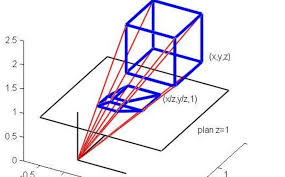
\includegraphics[scale=0.65]{pp.jpeg}
    \caption{Homogeneous Coordinates}
    \label{k}
\end{figure}

We shall introduce the concept with a transformation from the 2D Euclidean space to the 2D projective space.

A normal 2D point with the form
\[\mathbf{x} = \begin{bmatrix}
    x \\ y
\end{bmatrix}\]

in projective space becomes
\[\tilde{\mathbf{x}} = \omega \begin{bmatrix}
    x \\ y \\ 1
\end{bmatrix} = \omega \overline{\mathbf{x}}\]

To perform translation, we use the following formula, 
\[{\mathbf{x}}' = \begin{bmatrix}
    I &t
\end{bmatrix} \overline{\mathbf{x}}\]

or equivalently, 
\[{\mathbf{x}}' = \begin{bmatrix}
    I &t \\
    0^T &1 \\
\end{bmatrix} \overline{\mathbf{x}}\]

A rigid motion is defined by a translation combined with a rotation. With the translation we already defined above, we will have

\[{\mathbf{x}}' = \begin{bmatrix}
    R &t
\end{bmatrix} \overline{\mathbf{x}}\]

where 
\[{\mathbf{R}} = \begin{bmatrix}
    cos(\theta) &-sin(\theta) \\
    sin(\theta) &cos(\theta) \\
\end{bmatrix}\]

Affine transformation is another type of transformation common with homogeneous coordinates, and it is given by:

\[\mathbf{x}' = \begin{bmatrix}
    a_{00} &a_{01} &a_{02} &a_{03} \\
    a_{10} &a_{01} &a_{12} &a_{13} \\
    a_{20} &a_{11} &a_{22} &a_{23} \\
    a_{30} &a_{21} &a_{32} &a_{33} \\
\end{bmatrix} \overline{\mathbf{x}}\]

Under affine transformations, parallel lines and planes remain parallel.

\subsection{Coordinates}

Suppose we have a system of coordinates in a room with axes $\mathbf{X_r,Y_r,Z_r}$ and some point $P$ with coordinates $(X_r, Y_r, Z_r)$. Of course, the camera will not always be at the origin of this coordinate system, so we must create a new coordinate system for the camera. Call the axes of this new coordinate system $\mathbf{X_c,Y_c,Z_c}$. 
Then we can transform our ``room coordinates'' into ``camera coordiantes'' by a rotation composed with a translation. Suppose this rotation is given by a matrix $M$ and the translation is given by a vector $v$. Then the new coordinates $P$ of the point $P$ are 
\[
\begin{bmatrix}
    X_c \\
    Y_c \\
    Z_c
\end{bmatrix} = M \begin{bmatrix}
    X_r \\
    Y_r \\
    Z_r
\end{bmatrix} + v
.\]

To make this notation more compact, we may also write this using an augmented matrix as
\[
\begin{bmatrix}
    X_c \\
    Y_c \\
    Z_c
\end{bmatrix} = \begin{bmatrix}
    M & v
\end{bmatrix}
\begin{bmatrix}
    X_r \\
    Y_r \\
    Z_r \\
    1
\end{bmatrix}
.\] Here's an image for what is happening so far. 

\begin{center}
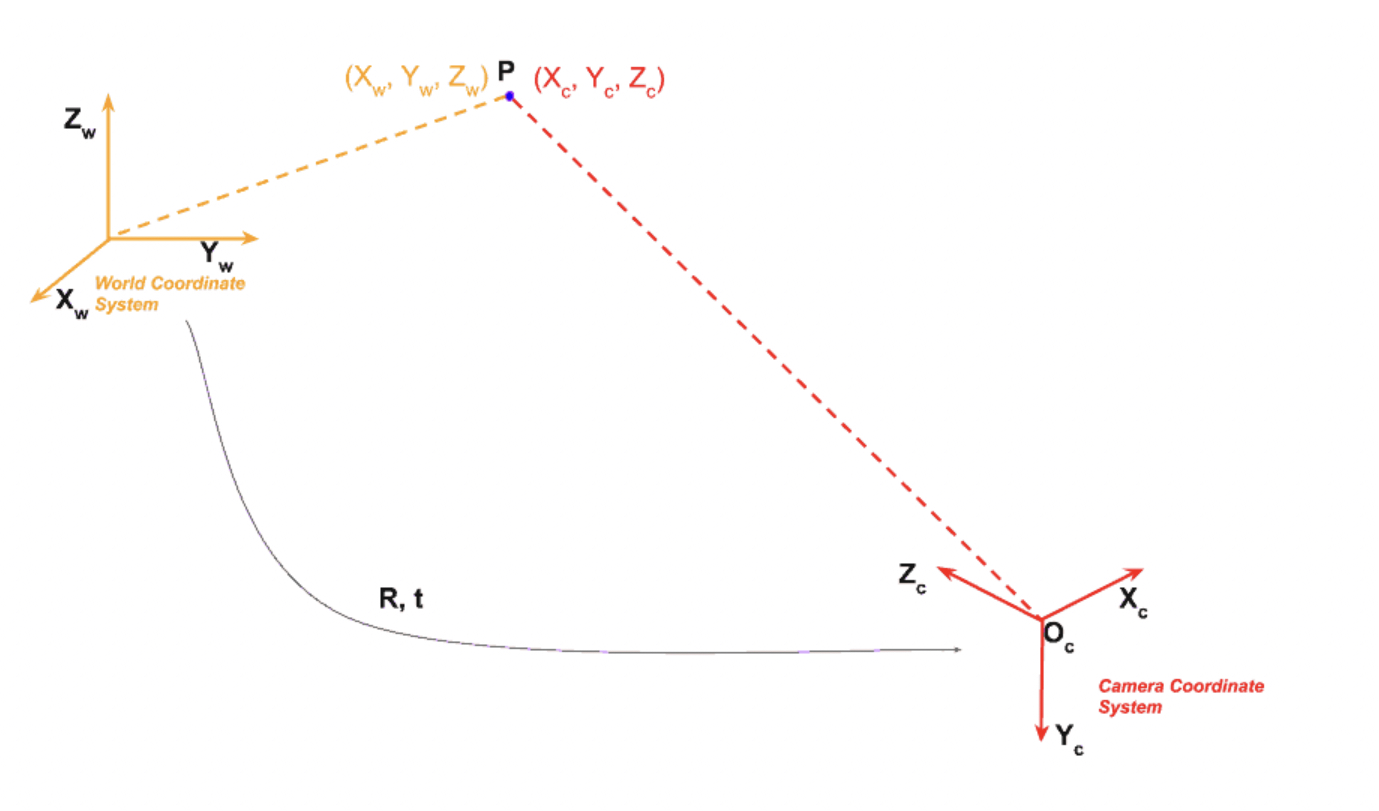
\includegraphics[scale=0.3]{IMG_1112.jpeg}
\end{center}

Now that we've established this coordinate system, we are ready to project our coordinates onto a plane to form our image. 

\subsection{Projecting onto the Plane}
We will try to obtain coordinates $(x,y)$ as follows.

\begin{figure}[h]
    \centering
    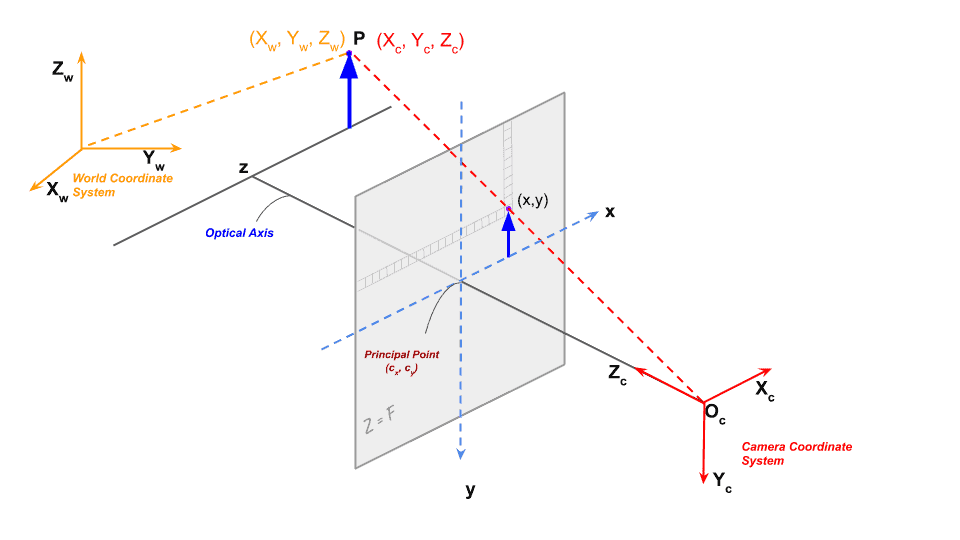
\includegraphics[scale=0.4]{IMG_1110.png}
    \caption{Caption}
    \label{fig:enter-label}
\end{figure}


We now go about doing this. Call the origin of our camera coordinate system $O_c$, called the \textit{optical center}. Suppose the plane we are projecting onto is a distance $F$ away from $O_c$. We see that the new point $P'$ we project onto has coordinates (with respect to the axes of our camera coordinate system) $(x,y,f)$. By using similar triangles, we find that $x = f\frac{X_c}{Z_c}$ and $y= f\frac{Y_c}{Z_c}$. Letting $x' = xZ_c$, $y' = yZ_c$, and $z' = Z_c$, we can write the following:
\[
\begin{bmatrix}
    x' \\
    y' \\
    z'
\end{bmatrix} = \begin{bmatrix}
    f & 0 & 0 \\ 
    0 & f & 0 \\
    0 & 0 & 1 
\end{bmatrix}\begin{bmatrix}
    X_c \\
    Y_c \\
    Z_c
\end{bmatrix}
.\] The matrix $\begin{bmatrix}
    f & 0 & 0 \\
    0 & f & 0 \\
    0 & 0 & 1 
\end{bmatrix}$ is called the \textit{intrinsic} matrix because it contains the intrinsic parameters of the camera (namely, the focal length). There are some problems with this model, however.
\begin{itemize}
    \item The pixels in the image sensor may not be square, and so we may have two different focal lengths $f_x$ and $f_y$.
    \item The optical center $(c_x, c_y)$ of the camera may not coincide with the center of the image coordinate system.
    \item There may be a small skew $\gamma$ between the x and y axes of the camera sensor.
\end{itemize}

To adjust for these possible problems, we modify the intrinsic matrix to become
\[\begin{bmatrix}
    f_x & \gamma & c_x \\
    0 & f_y & c_y \\
    0 & 0 & 1
\end{bmatrix}.\]

\section{Lens Distortion}
So far, we have developed the \textbf{pinhole model}. This means we assumed the aperture through which light passes into the camera is very small. This has the advantage that images taken are clear and sharp. However, less light can pass through the hole, giving a darker image. To deal with this problem, we replace the pinhole by a lens. This allows more light rays to pass through the hole, and because of the optical properties of the lens, we get a focused image. The image also becomes brighter. Unfortunately this doesn't solve all of our problems. 


\subsection{Radial and Tangential Distortion}

There are two main kinds of lens distortion, namely \textbf{radial distortion} and \textbf{tangential distortion}. 

Radial distortion occurs due to the unequal bending of light. Light rays bend more closer to the edges of the lens than center. This has the effect of making straight lines look curved. 

The rays bend more near the edges of the lens than the rays near the centre of the lens. Due to radial distortion straight lines in real world appear to be curved in the image. The light ray gets displaced radially inward or outward from its ideal location before hitting the image sensor. There are two types of radial distortion effects. First, there is \textbf{barrel distortion}, corresponding to negative radial displacement. Then there is \textbf{pincushion distortion}, which corresponds to positive radial displacement. The figure below, although a bit exaggerated, should clarify.

\newpage 
\begin{figure}[h]
\centering
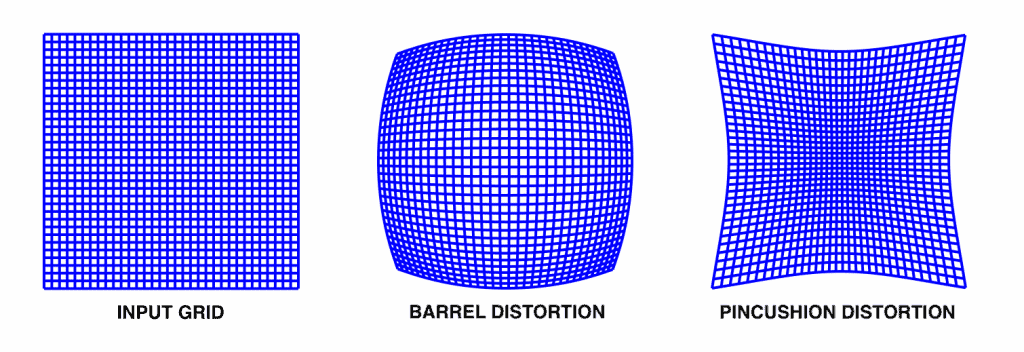
\includegraphics[scale=0.37]{Distortion.png}
\caption{Examples of barrel and pincushion distortion}
\end{figure}

Tangential distortion, on the other hand, is a sort of ``decentralizing'' effect. It occurs due to misalignments in the camera lens with respect to the image sensor or film plane. An exaggerated example tangential distortion is as follows.

\begin{figure}[h]
    \centering
    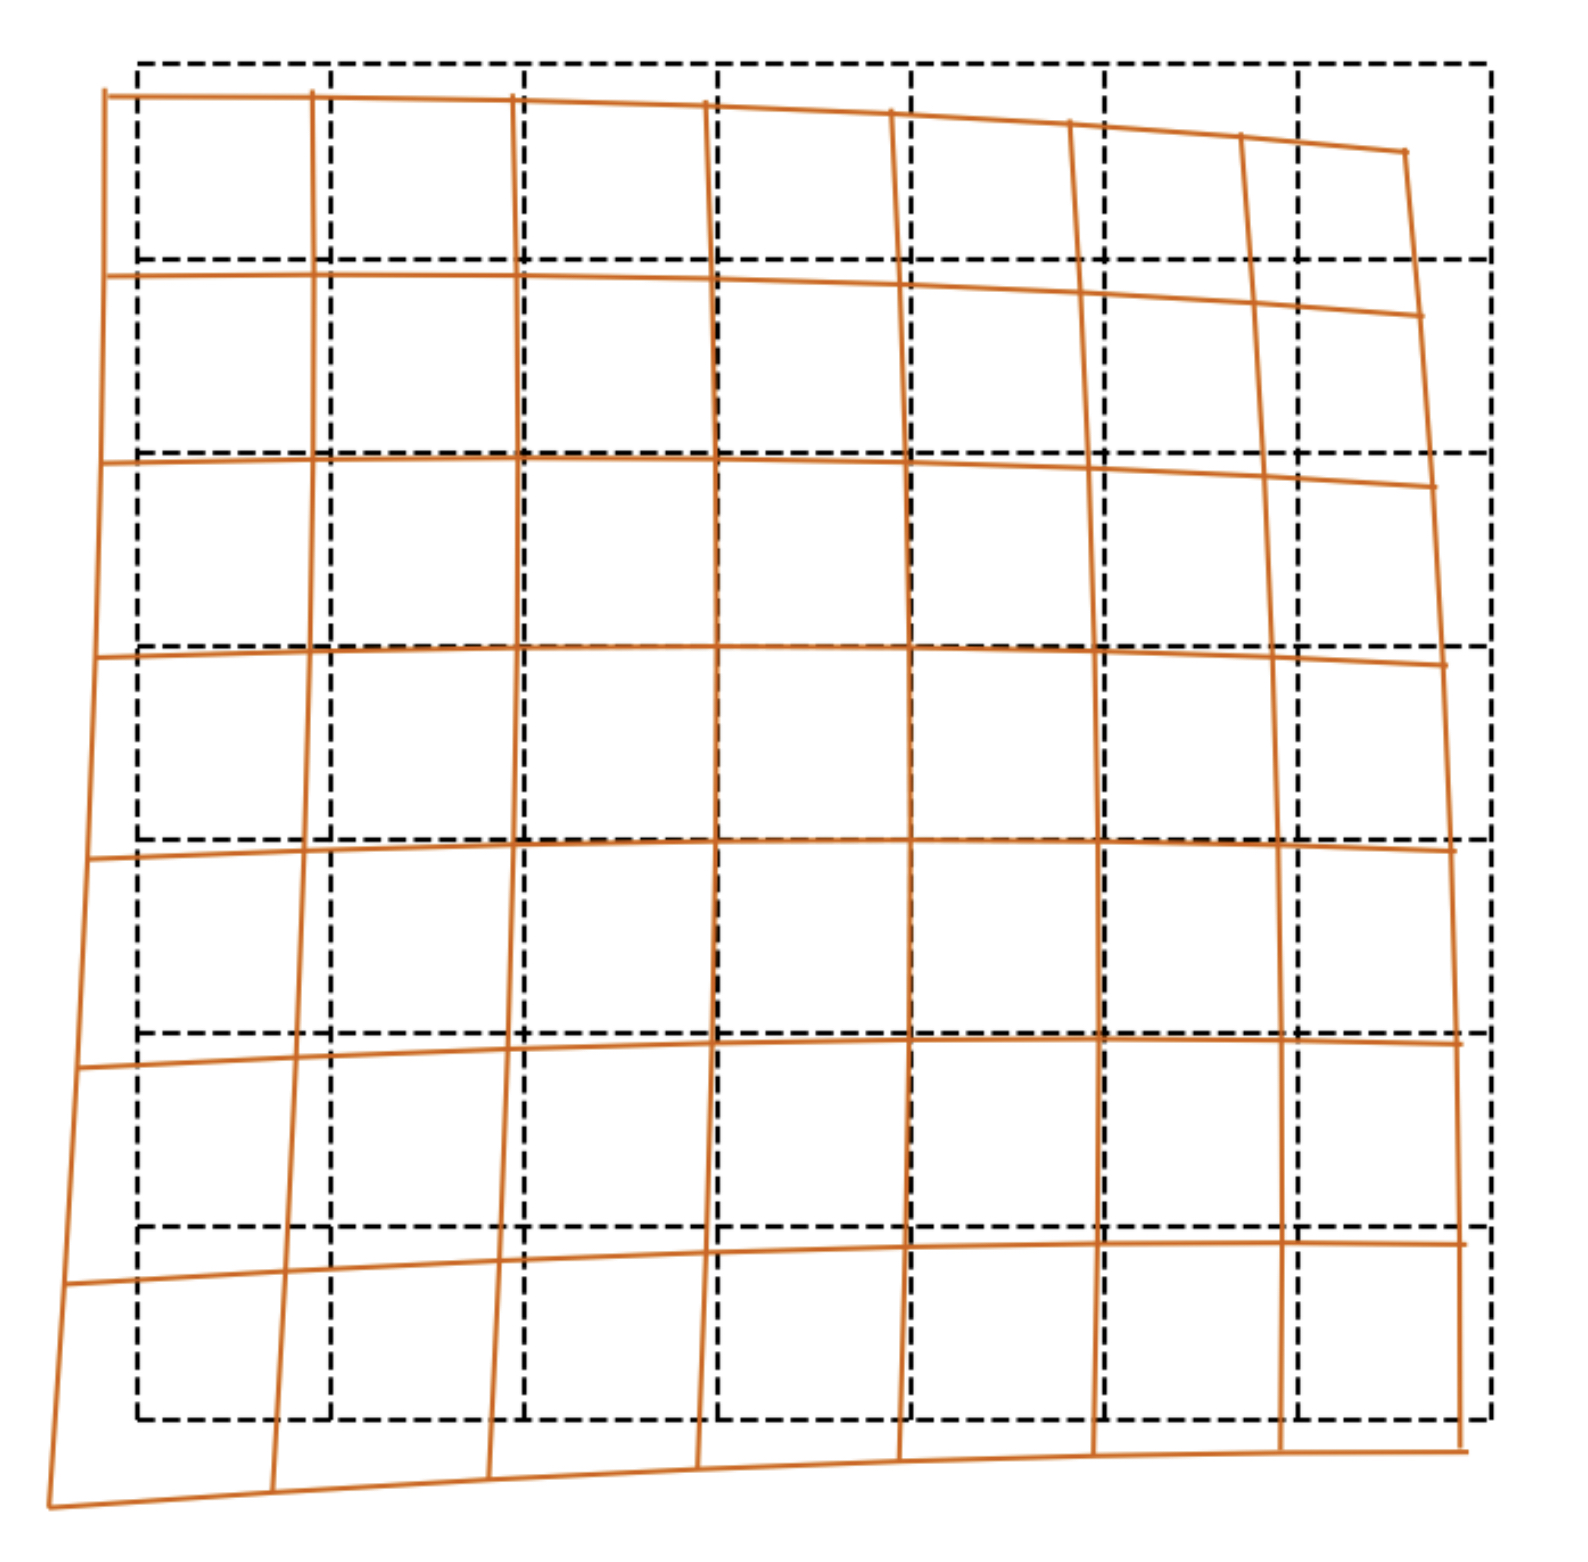
\includegraphics[scale=0.1]{IMG_1106.jpeg}
    \caption{Extreme tangential distortion}
    \label{fig:enter-label}
\end{figure}

In terms of the lens itself and how it fails to align with the image plane, here is a picture illustrating that. 

\begin{figure}
    \centering
    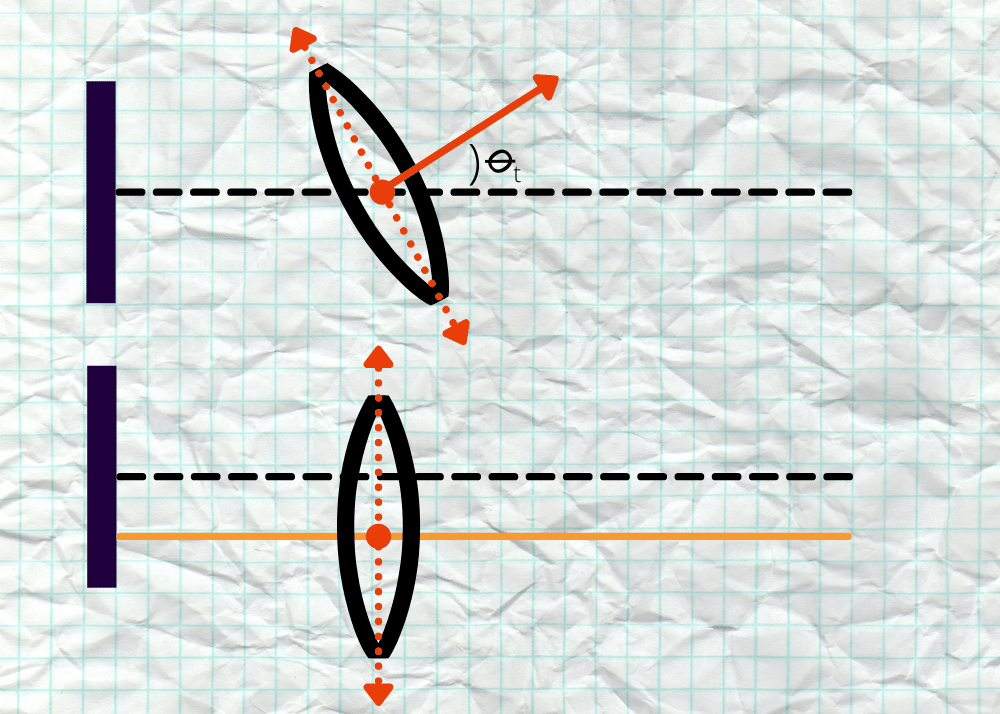
\includegraphics[scale=0.2]{Images/IMG_1138.png}
    \caption{Lens failing to align with image plane}
    \label{aael}
\end{figure}

\newpage

It is of course possible to have both tangential and radial distortion. This is called \textbf{compound distortion}.

\begin{figure}[h]
    \centering
    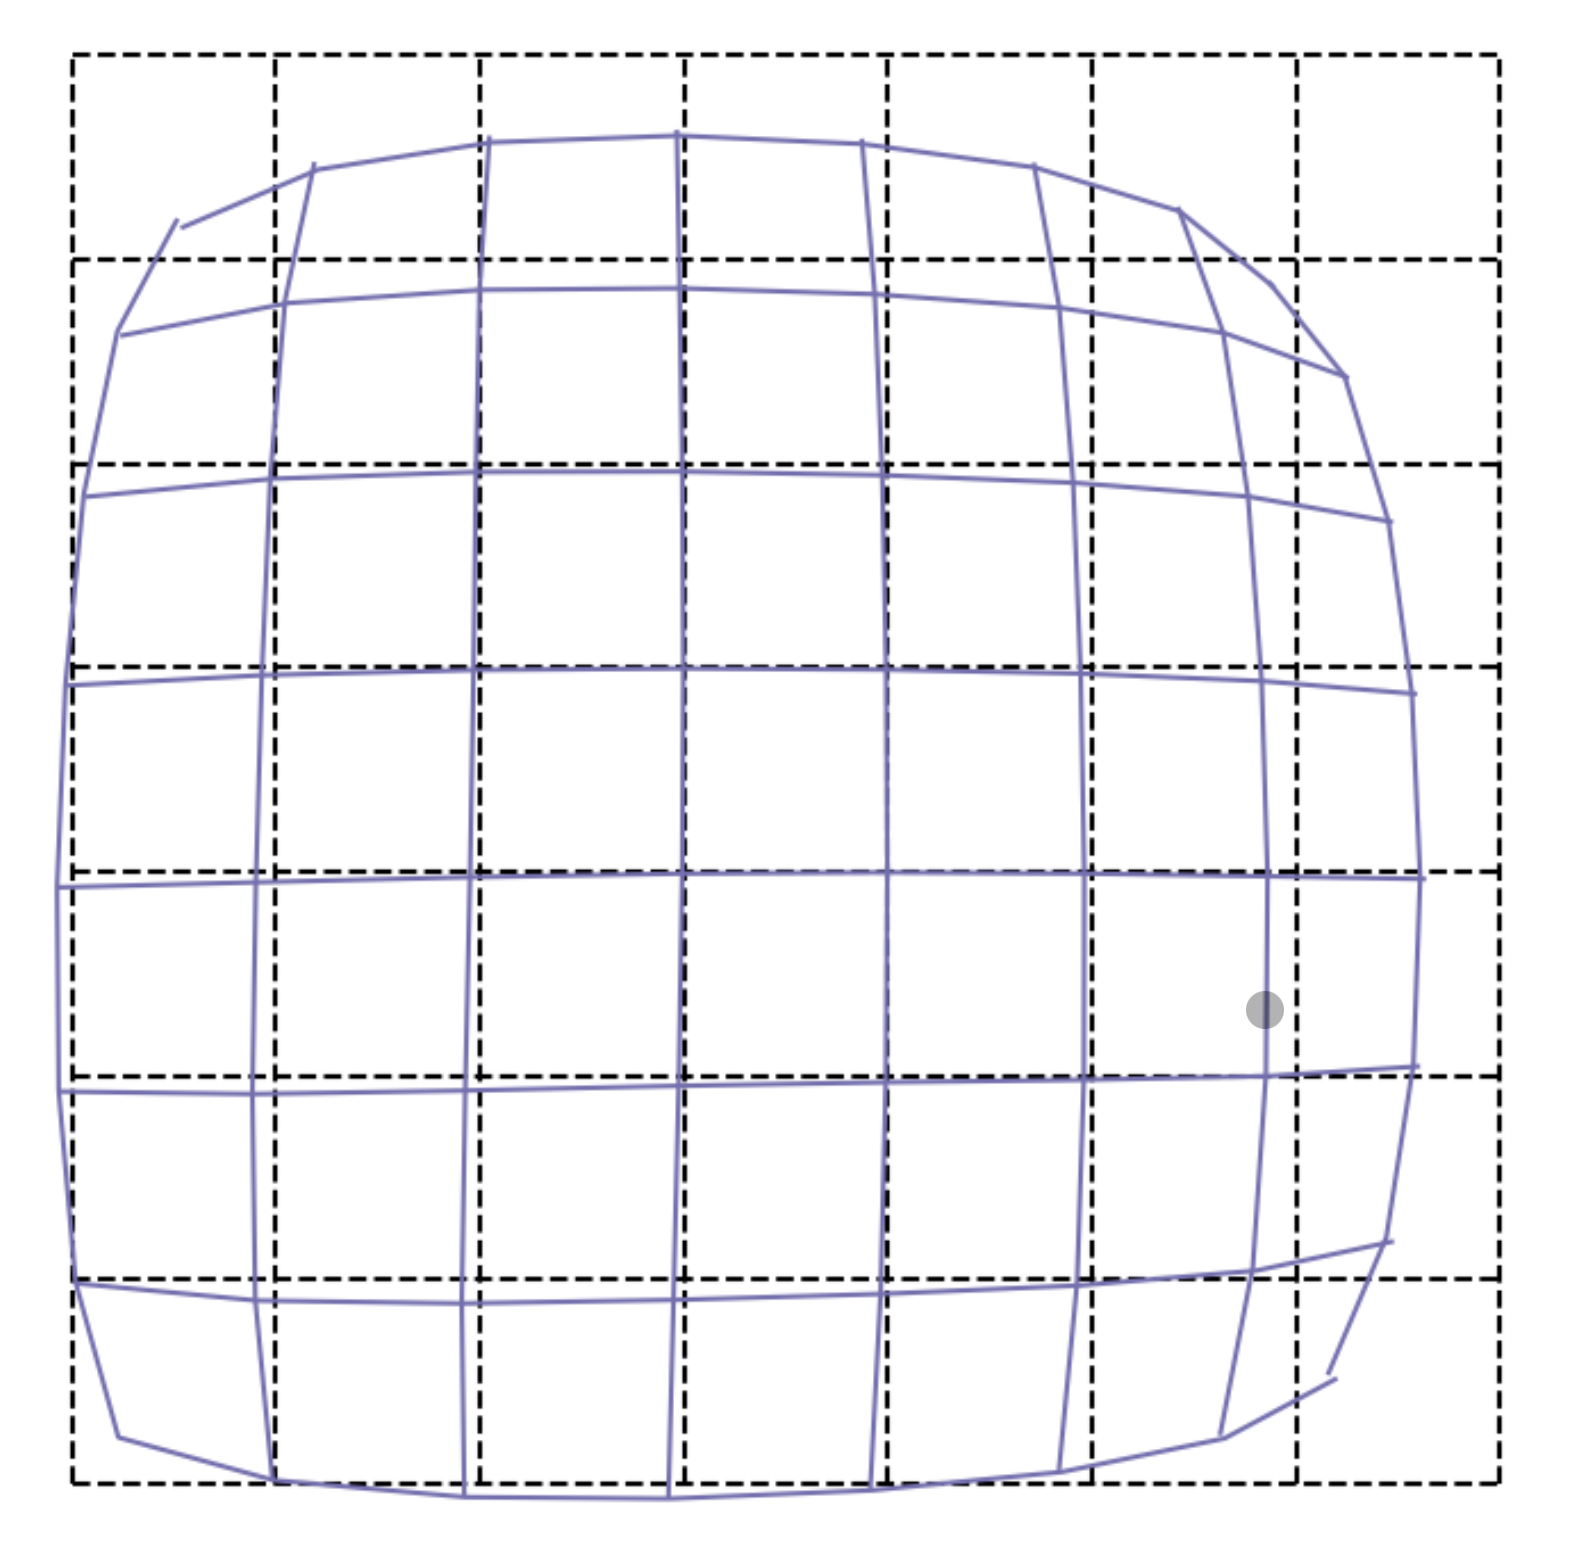
\includegraphics[scale=0.1]{IMG_1108.jpeg}
    \caption{Extreme compound distortion}
    \label{l}
\end{figure}
Okay, great. We have all these problems. How can we solve them?

\subsection{Mathematically Modeling Lens Distortion}

Before we actually modify our model for the pinhole (ie. actually find the distortion $\gamma$), we first need to talk about camera calibration. Recall the intrinsic matrix we derived in section 1. 
\[
K = \begin{bmatrix}
    f_x & \gamma & c_x \\ 0 & f_y & c_y \\ 0 & 0 & 1
\end{bmatrix}
.\] The goal of camera calibration is to find this matrix when given an image, as well as the rotation matrix and translation vector we talked about when going form ``world coordinates'' to ``camera coordinates''. In summary, we input a collection of images whose 2D image coordinates and 3D world coordinates are known, and we spit out the matrix $K$ and the rotation and translation vector. 

\begin{itemize}
    \item [Step 1: ] First we take a picture of a chessboard on a wall. We define ``world coordinates'' using the chess board attached in our image. We choose any corner of the chessboard to be our origin for this coordinate system. We pick the $\mathbf{x}$ and $\mathbf{y}$ axes to be along the wall while the $\mathbf{z}$ axis is perpendicular to the wall.  We then define the other coordinates of points on the wall with respect to this origin. Note that all points on the checkerboard have $\mathbf{z}$-coordinate equal to 0.

    Also, a side remark. Chess boards are used very often in computer vision because they are easy to identify. 
    \item [Step 2: ] Second, we take pictures of the chess board from different angles. Of course, this depends on how much control we have over the process, but in this paper we assume a certain degree of control over the process. 
    \item [Step 3: ] In step 1, we defined the coordinates of the other parts of the chess board with respect to the origin. But how do we actually compute them? Luckily, OpenCV has a feature called \code{findChessboardCorners}. Of course, we want to make this precise. To do this, we use OpenCV's function \code{cornerSubPix}. This function takes the original image and the location of the corners. It then looks for the best corner location inside a small a small ball around the corners.
    \item [Step 4: ] We use OpenCV's \code{cameraCalibrate} method. The math behind the implementation is rather lengthy, but the general idea is that we solve a nonlinear optimization problem that minimizes the difference (reprojection error) between the observed 2D image points and the 3D points projected onto the image plane using the estimated parameters. The interested reader may read more about this in \cite{zhangmethod}.
\end{itemize}

Now we can finally modify our model. The camera calibration process we described above finds both intrinsic and extrinsic parameters. This helps us modify our model as follows.

\begin{align*}
    \gamma &= \frac{1 + K_1r^2 + K_2r^4 + K_3r^6}{1+K_4r^2 + K_5r^4 + K_6r^6} \\
    r^2 &= x'^2 + y'^2 \\
    x'' &= x'\cdot\gamma + 2P_1x'y' + P_2(r^2+2x'2) \\
    y'' &= y'\cdot\gamma + P_1(r^2 + 2y'^2) + 2P_2x'y' \\
\end{align*}

where $x''$ and $y''$ are the new 2-dimensional coordinates in our image. The coefficients $K_1, \ldots, K_6$ represent radial distortion and the coefficients $P_1, P_2$ represent tangential distortion. The direct implementation in the code is talked about more in section 3. 

The interested reader might be wondering how on earth we got these formulas for $\gamma$. We get them from the Brown-Conrady model. This model characterizes radial distortion as a series of higher order polynomials. Namely, they say that 
\[
r = \sqrt{x^2 + y^2} \qquad \delta r = k_1r^3 + k_2r^5 + k_3r^7 + \ldots 
.\] Where $r$ is of course the distance of the points from the origin, and $\delta r$ is the change in $r$ after the distortion happens. Notice that the new radius, say $r'$, is $r+\delta r$.

In practice, only the first three terms of this formula are used. In fact, for cameras with lens systems that are simpler than usual, it suffices to use the first two terms. Anyway, similar power series can also model $x$ and $y$, and $\gamma$ is a measure of the proportional distortion between $x$ and $y$. Thus we get the formula above. 

One might still wonder how they got this characterization. It seems to be from empirical evidence. Brown and Conrady observed that the distortion was a function of the radial distance of each point. Functions in nature tend to be nice (ie. differentiable), so we can mostly differentiate this function. Thus we can sort of approximate it with a power series, which is what the above shows. 

So far, we have considered mainly \textit{symmetric} radial distortion. That is, we have only considered radial distortion where the distortion depends only on the radial distance from the origin. There are also \textit{asymmetric} radial distortions, where the distortion depends on both radial distance and the distance of the object being photographed. This type of distortion is actually more pronounced in the images in two cases:
\begin{enumerate}
    \item Cameras that have long focal length and short relative objective distances. These enlarge the effect of antisymmetric radial distortion because their lens' are often very complicated, introducing geometric complexities and leading to aberrations. 
    \item When the light comes through a medium with high refraction. 
\end{enumerate}

Thankfully, neither of these situations is very likely, so we do not consider them in this paper. 


\section{The algorithm}

In order to calibrate our camera in a real world setting, we would first need to have stack of images taken from different angles and planes. And each of these images need to have a chessboard pattern in them. The chessboard pattern should be a grid of squares, and it's usually recommended that the squares be as close to perfect squares as possible. This means that the width of a square should be roughly the same as its height.

\begin{figure}[h]
    \centering
    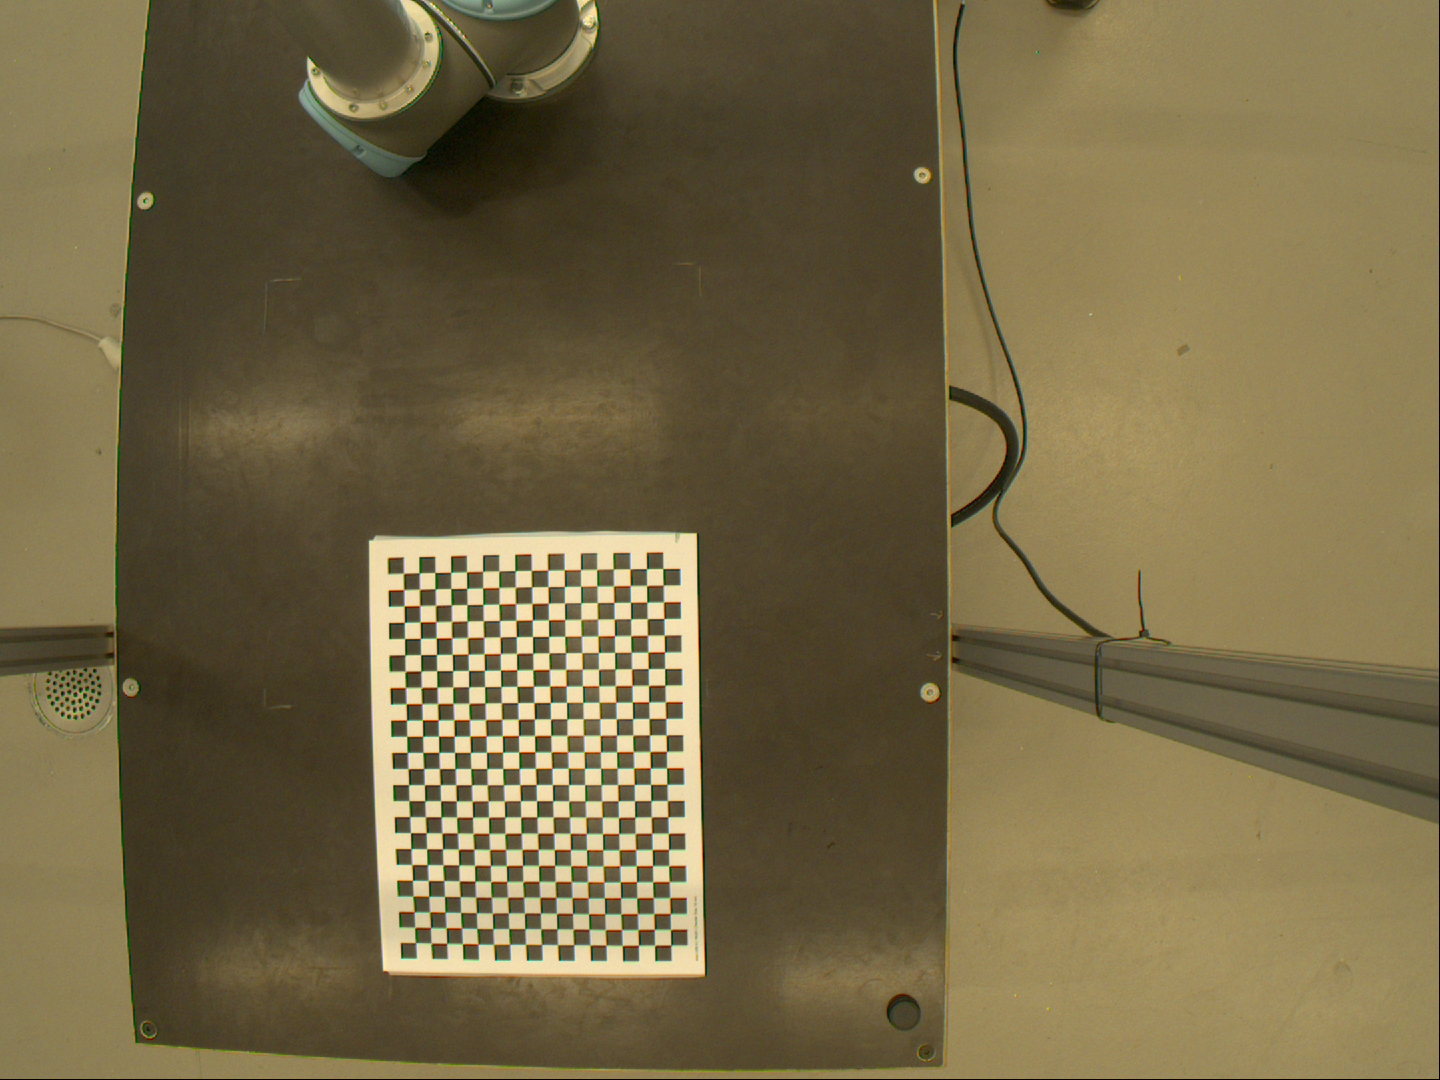
\includegraphics[scale=0.12]{cali1.png}
    \caption{Original image}
    \label{k}
\end{figure}


With the acquired images, we proceed to construct two lists of points for camera calibration.

The first list, named \code{objpoints} (short for object point), is meant to capture the spatial coordinates of the chessboard corners in the real world, or the distances between the squares on the physical chessboard, which is then translated into a structured 2D array of points. These object points serve as a representation of the true geometry of the chessboard, allowing the calibration process to establish a connection between the camera's perspective and the real-world coordinates.

In contrast, the second list, named \code{imgpoints}, is designed to house the pixel coordinates of the chessboard corners as they appear in the captured images. This list is generated through the utilization of OpenCV's corner detection method (\code{findChessboardCorners}), which identifies and records the precise location of the chessboard corners within the images. 

These two lists facilitates the calibration process by enabling the estimation of the camera's intrinsic and extrinsic parameters, bridging the gap between the physical world and the digital image. Hence, the camera will be precisely calibrated, laying the foundation for a wide array of applications in computer vision, 3D reconstruction, and image processing.

\begin{figure}[h]
    \centering
    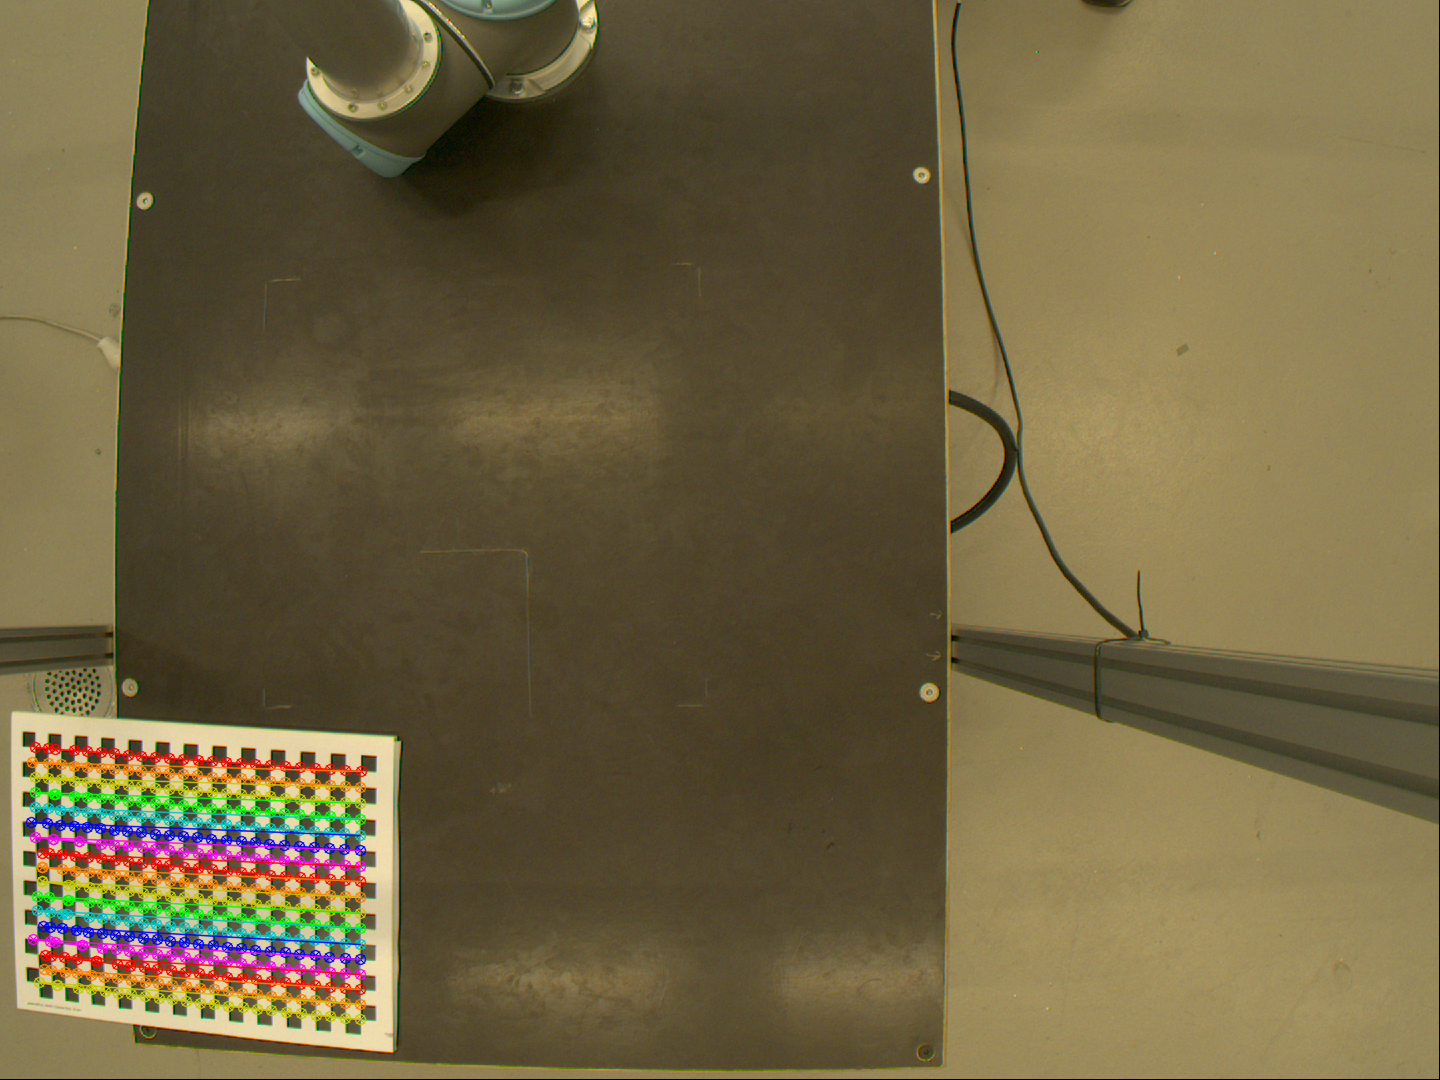
\includegraphics[scale=0.12]{process1.png} \qquad 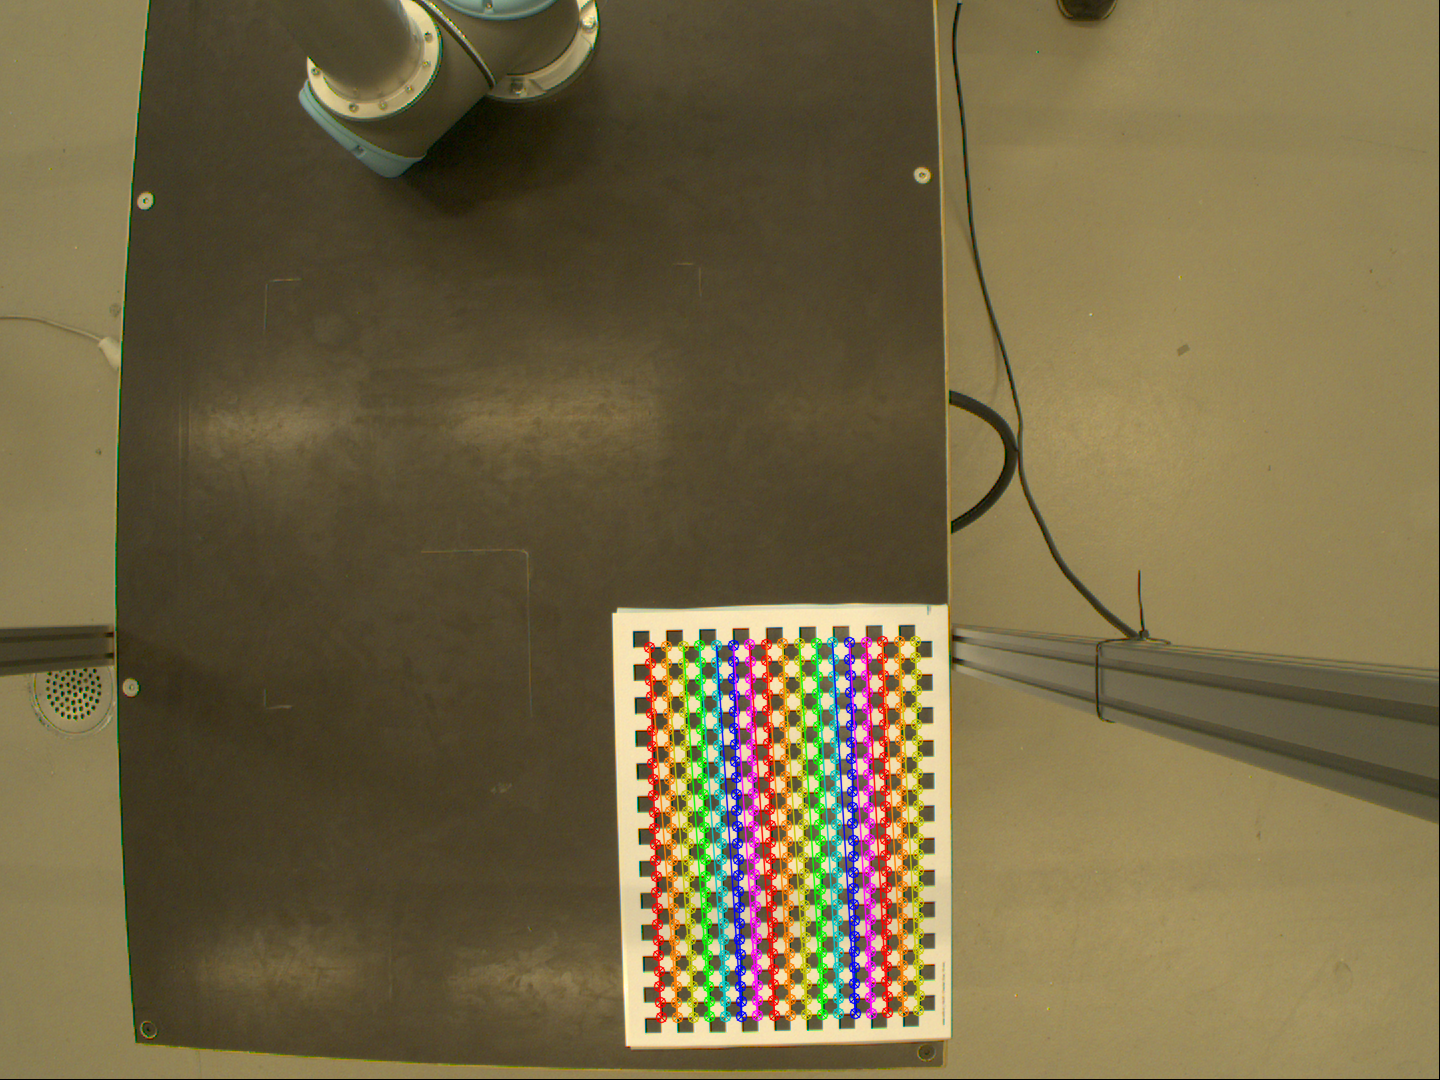
\includegraphics[scale=0.12]{Images/process2.png}
    \caption{Corner detection at work}
    \label{k}
\end{figure}

% Please put process2 side by side thankkkk

The next step in the calibration process requires us to translate the 3D points we attained through calculations and the 2D points we attained through image recognition of the chessboard. This translation is rooted in principles of perspective projection, relying on the camera's intrinsic properties and its position relative to the chessboard.

To simplify and expedite this task, we employ OpenCV's "cameraCalibration" method. By feeding it the pairs of "objpoints" and "imgpoints," we obtain critical camera parameters. These include the camera matrix, which encapsulates intrinsic characteristics, distortion coefficients to correct optical imperfections, and rotation and translation vectors describing the camera's orientation and position relative to the chessboard.

Next, we calculate a new camera matrix that factors in the distortion using \code{getOptimalNewCameraMatrix}. Using this new camera matrix, we can call the \code{undistort} method OpenCV provides.

The next step involves calculating a modified camera matrix that corrects for lens distortion. OpenCV provides a helpful function called \code{getOptimalNewCameraMatrix} for this purpose. This refined camera matrix not only addresses distortions but also optimizes it for the specific region of interest in the image.

Once we have this new camera matrix, we can proceed to use OpenCV's \code{undistort} method. This method effectively removes lens distortions from the images, ensuring they are geometrically accurate and free from optical aberrations. 


\begin{figure}[h]
    \centering
    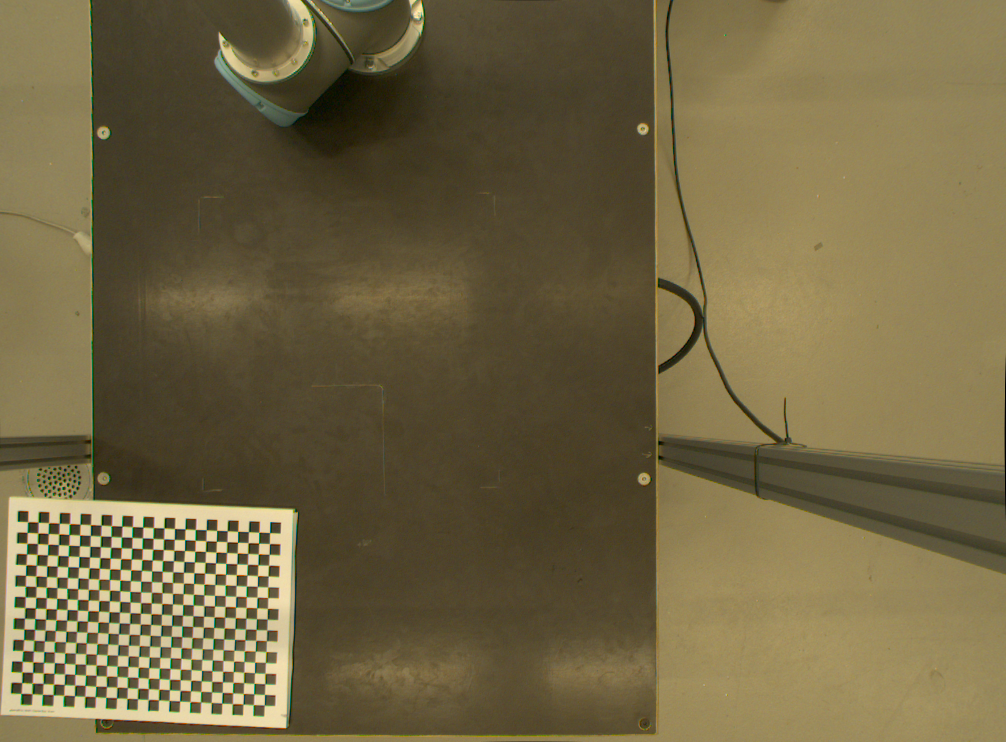
\includegraphics[scale=0.18]{Images/caliResult3.png}\qquad 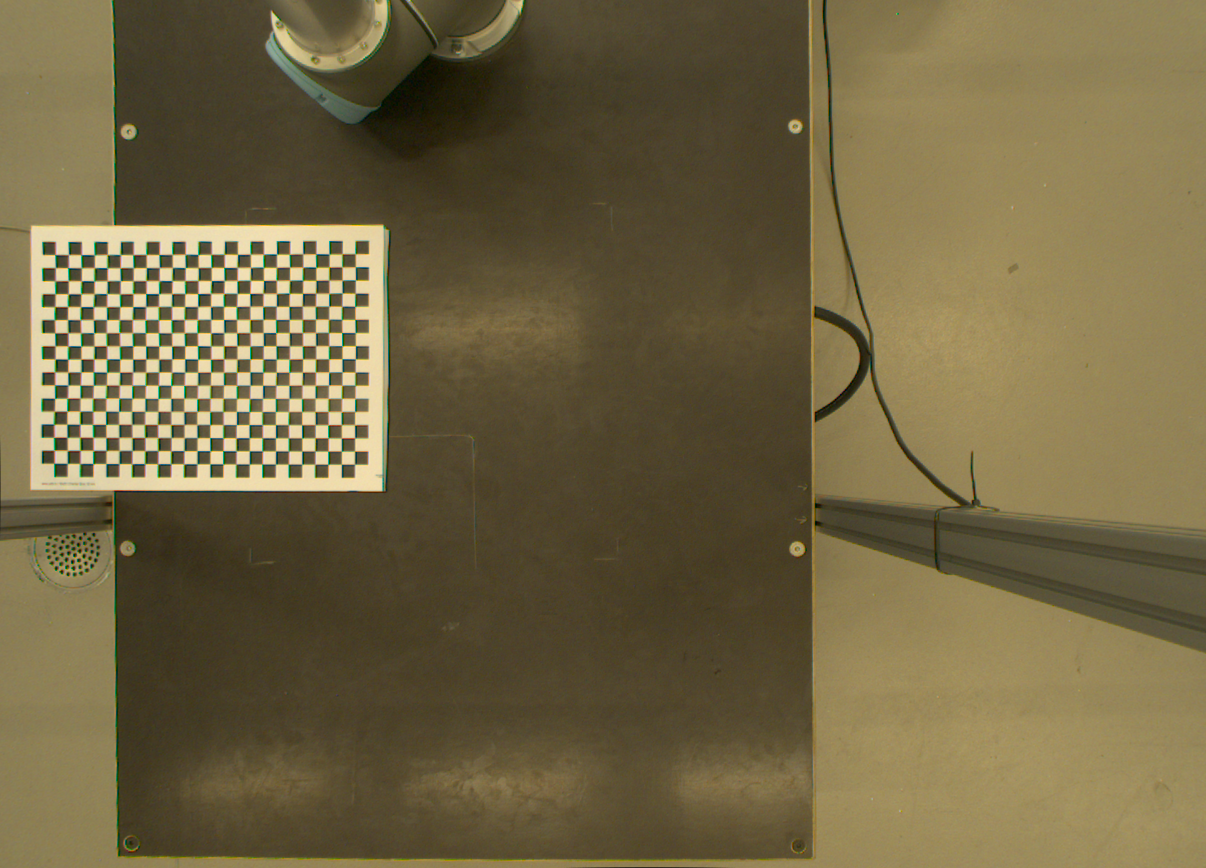
\includegraphics[scale=0.15]{Images/caliResult4.png}
    \caption{Undistorted image}
    \label{kk}
\end{figure}

% Please put result4 side by side thankkkk

In the final phase of the calibration process, we will assess the accuracy of the distortion coefficients. This evaluation is carried out by projecting the 3D object points onto the 2D image plane, but this time using our calculated camera matrix and distortion coefficients. The procedure essentially involves establishing a set of equations, with the distortion coefficients as the variables to be determined and the object points as known entities.

The optimization is achieved by minimizing the differences between the calculated and observed points, with the aid of an absolute norm. The variations across all images in the stack are carefully measured, and the results are averaged. This  assessment serves as a vital quality control step, ensuring that the calibration parameters yield accurate and consistent results across the entire dataset, further enhancing the reliability of the camera calibration process.


\begin{figure}[h]
    \centering
    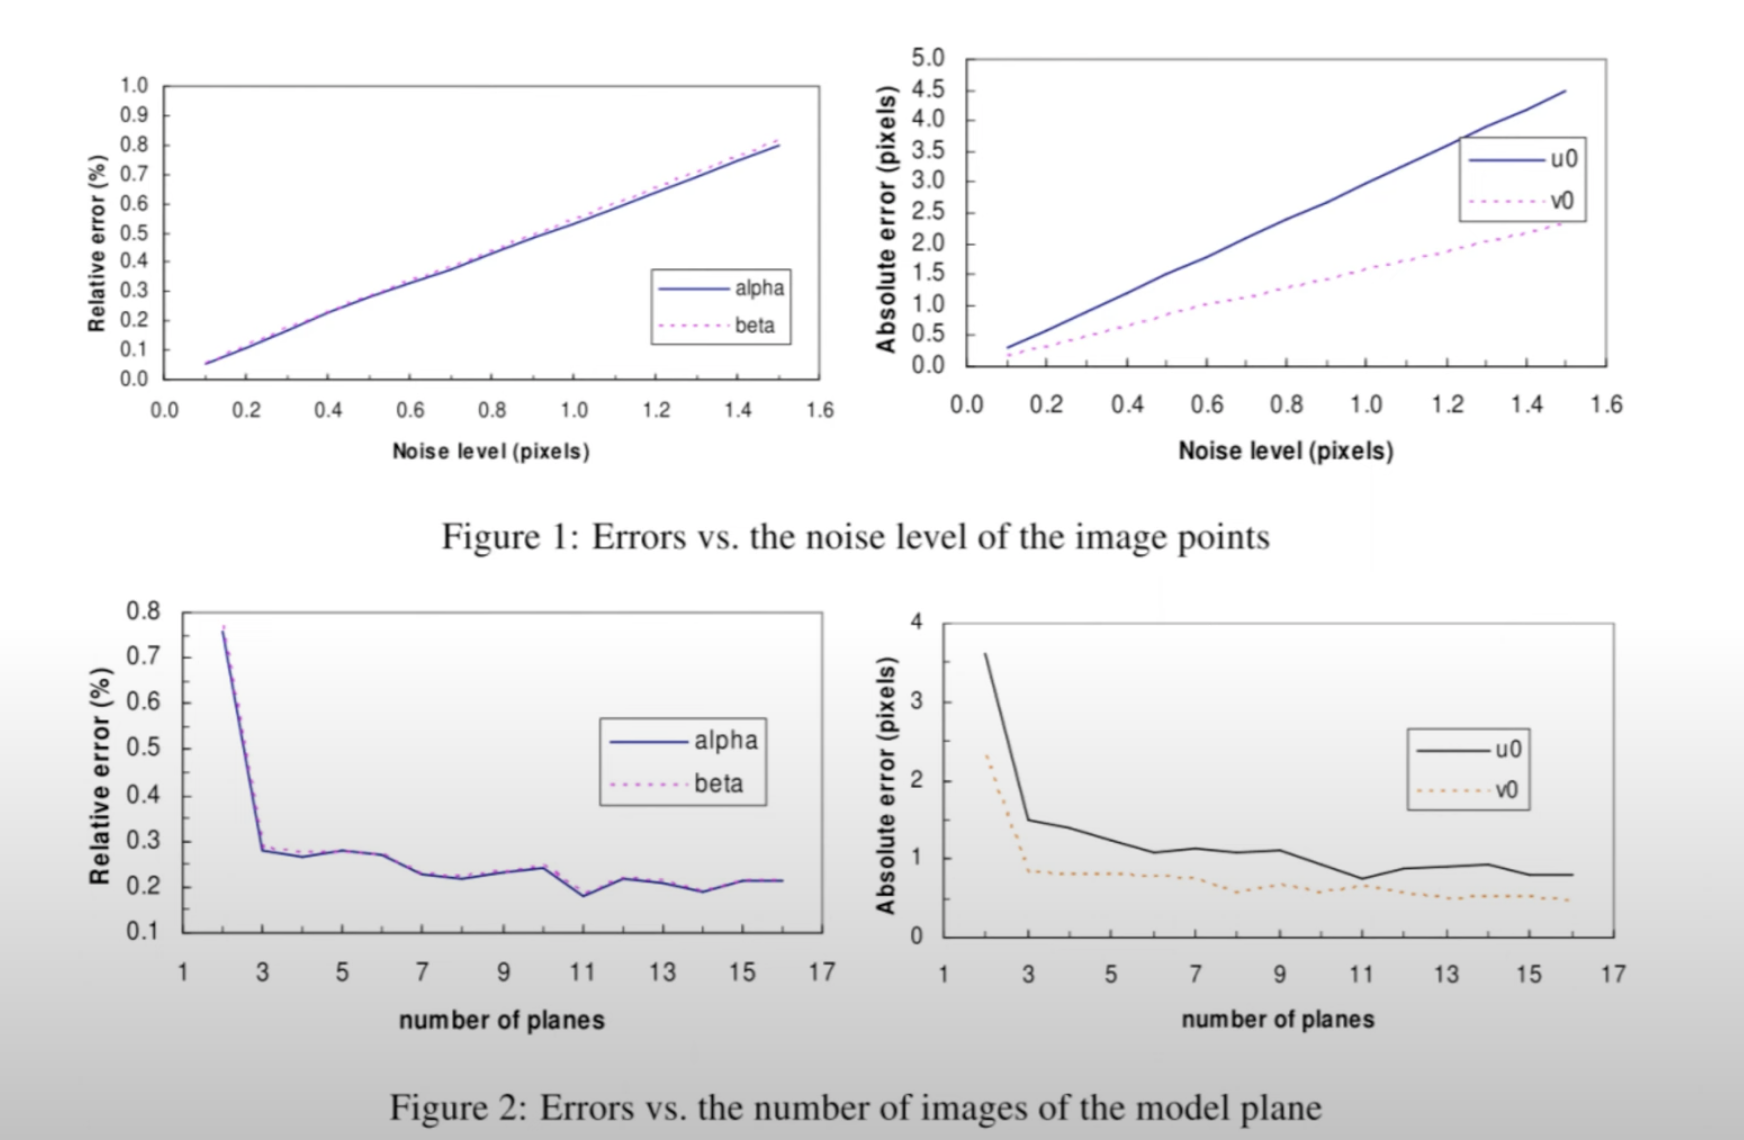
\includegraphics[scale=0.2]{Images/Screen Shot 2023-10-21 at 1.09.31 PM.png}
    \caption{Error analysis}
    \label{k}
\end{figure}

One intriguing observation worth highlighting is that the quantity of images used in the calibration process doesn't always correlate with a reduction in error. In fact, a noteworthy aspect of this calibration endeavor is that the optimal range of images typically falls within the modest bracket of 5 to 15.

It may seem counterintuitive, but there's a rationale behind this phenomenon. Beyond a certain point, the inclusion of additional images doesn't significantly enhance the precision of the calibration parameters. Instead, it can introduce noise and computational complexity without commensurate improvements in accuracy.

The sweet spot of 5 to 15 images strikes a balance between acquiring a robust dataset for calibration and avoiding the pitfalls of overcomplicating the process. It provides an adequate number of data points to ensure accuracy while keeping the workflow manageable and efficient. This observation underscores the importance of a balanced approach in camera calibration, where quality and relevance of data take precedence over sheer quantity.



\nocite{*}
\printbibliography

\end{document}
